\documentclass[11pt]{article}
\usepackage[margin=2.1cm]{geometry}
\usepackage{amsmath,amssymb,booktabs,microtype}
\usepackage{xcolor}
\usepackage{tikz}
\usepackage{pgfplots}
\pgfplotsset{compat=1.18}
\usetikzlibrary{arrows.meta,positioning,fit,backgrounds,calc,shapes.geometric,decorations.pathreplacing}
\usepackage[colorlinks=true,linkcolor=nagblue,urlcolor=nagblue]{hyperref}

\definecolor{nagblue}{HTML}{2E5E8C}
\definecolor{naggreen}{HTML}{2E7D32}
\definecolor{nagorange}{HTML}{E8710A}
\definecolor{naggrey}{HTML}{9E9E9E}
\definecolor{lightg}{HTML}{E8F5E9}
\definecolor{lighto}{HTML}{FFF3E0}
\definecolor{lightb}{HTML}{E3F2FD}
\definecolor{lightr}{HTML}{FFEBEE}

\tikzset{
  box/.style={draw, rounded corners=2pt, align=center, inner sep=4pt, font=\small, minimum height=8mm},
  op/.style={box, fill=lightb, draw=nagblue},
  data/.style={box, fill=lightg, draw=naggreen},
  ord/.style={box, fill=lightr},
  lbl/.style={font=\footnotesize\itshape, text=black!60},
  fl/.style={-{Stealth[length=2mm]}, thick, draw=black!55},
}

\title{\textbf{Nagare}\\[2pt]\large A closed-form, MapReduce-parallel ML framework ---\\
what makes it fast, and how good it is}
\author{\texttt{github.com/kyberszittya/nagare}}
\date{2026-07-07}

\begin{document}
\maketitle

\begin{abstract}
\noindent Nagare (\emph{nagare}, ``flow'') is a Rust ML
framework that replaces the autograd tape and tensor-batch dispatch with
\emph{contiguous, auto-vectorised, closed-form kernels that MapReduce cleanly to
every CPU core}. On a fair CPU-vs-CPU forward it \emph{matches or beats} PyTorch
(a decade-tuned MKL-GEMM ecosystem) across a whole dimensionality sweep
(best-of-each $1.2$--$2.6\times$), on a static binary that uses $3$--$160\times$
less memory --- while its closed-form \emph{local} learner reaches
$\mathrm{AUROC}\approx1.0$ with $\sim47\times$ fewer parameters than
backpropagation on toy tasks. This document explains the exact mechanisms behind
both claims, and states honestly what is not yet proven.
\end{abstract}
% Note: remove the CJK line above if the CJK package is unavailable.

\section{What Nagare is}
Nagare is a \textbf{paradigm-native, closed-form} framework for
signed-hypergraph / point-set computation --- deliberately \emph{not} a tensor
autograd engine. Four design commitments:
\begin{enumerate}\itemsep1pt
  \item \textbf{Closed-form \((\text{forward},\text{backward})\) pairs, no tape.}
  Every operator is two plain Rust functions over flat \texttt{\&[f32]} buffers,
  with hand-derived analytic gradients --- no graph to build, traverse, or free.
  \item \textbf{Struct-of-arrays cycle pool} as the universal datum (contiguous,
  cache-friendly, no pointer chasing).
  \item \textbf{Multivector-valued gradients} (Clifford algebra), so the sign
  structure of signed graphs is first class.
  \item \textbf{MapReduce parallelism} over independent rows / cycles, not
  tensor-batch dispatch.
\end{enumerate}

\section{Architecture}
\begin{figure}[h]\centering
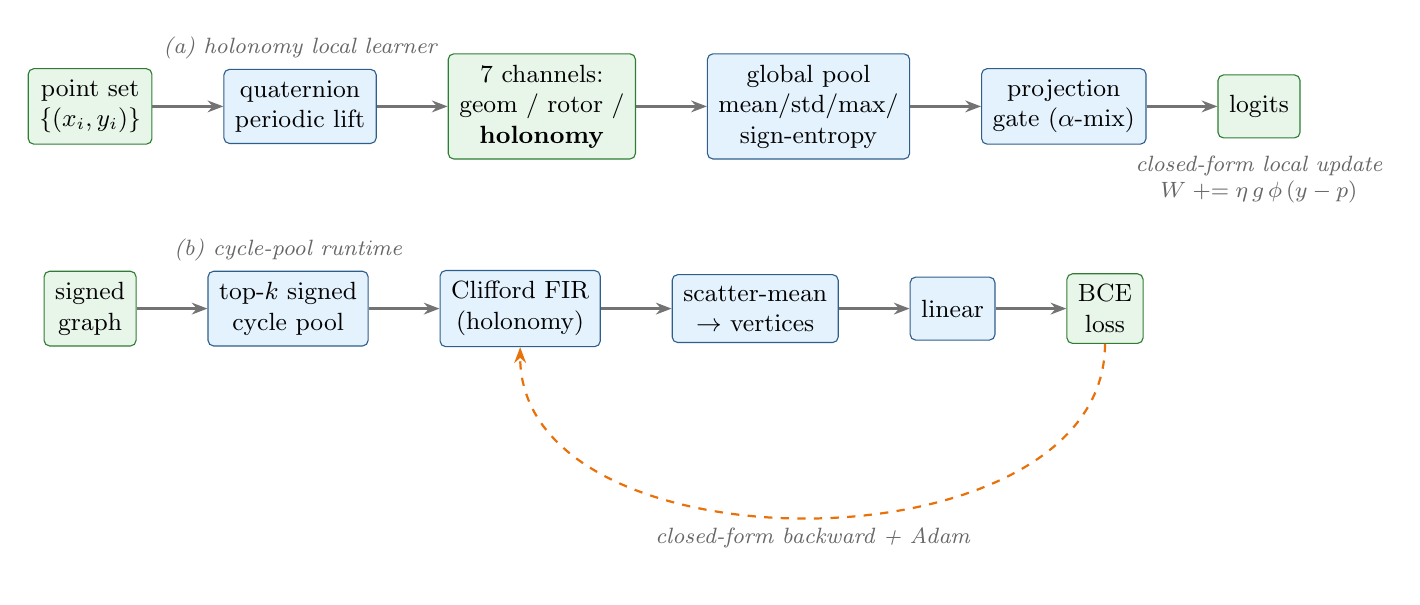
\begin{tikzpicture}[node distance=6mm and 9mm]
  % ---- (a) holonomy local learner ----
  \node[data] (pts) {point set\\$\{(x_i,y_i)\}$};
  \node[op, right=of pts] (lift) {quaternion\\periodic lift};
  \node[data, right=of lift] (ch) {7 channels:\\geom / rotor /\\\textbf{holonomy}};
  \node[op, right=of ch] (pool) {global pool\\mean/std/max/\\sign-entropy};
  \node[op, right=of pool] (gate) {projection\\gate ($\alpha$-mix)};
  \node[data, right=of gate] (out) {logits};
  \foreach \a/\b in {pts/lift,lift/ch,ch/pool,pool/gate,gate/out} \draw[fl] (\a)--(\b);
  \node[lbl, below=1mm of out, align=center] {closed-form local update\\$W \mathrel{+}= \eta\,g\,\phi\,(y-p)$};
  \node[lbl, above=0mm of lift] {(a) holonomy local learner};

  % ---- (b) cycle-pool runtime ----
  \node[data, below=16mm of pts] (g) {signed\\graph};
  \node[op, right=of g] (cyc) {top-$k$ signed\\cycle pool};
  \node[op, right=of cyc] (fir) {Clifford FIR\\(holonomy)};
  \node[op, right=of fir] (sc) {scatter-mean\\$\to$ vertices};
  \node[op, right=of sc] (lin) {linear};
  \node[data, right=of lin] (bce) {BCE\\loss};
  \foreach \a/\b in {g/cyc,cyc/fir,fir/sc,sc/lin,lin/bce} \draw[fl] (\a)--(\b);
  \draw[fl, dashed, draw=nagorange] (bce.south) to[out=-90,in=-90]
     node[lbl, below]{closed-form backward + Adam} (fir.south);
  \node[lbl, above=0mm of cyc] {(b) cycle-pool runtime};
\end{tikzpicture}
\caption{Two composition surfaces over the same closed-form kernels. Holonomy
(signed balance $=\mathbb{Z}_2$ holonomy) is the load-bearing signal in both.}
\end{figure}

Layers: \texttt{ops/} (forward+backward kernels: \texttt{linear},
\texttt{fused\_entropy\_update}, \texttt{project\_alpha\_mix},
\texttt{clifford\_fir}, \texttt{cayley\_rotor}, \texttt{fsr\_mixer},
Catmull--Rom/Chebyshev, \texttt{scatter}, \texttt{signed\_scatter}, \texttt{adam})
$\to$ \texttt{runtime} (cycle-pool composition) $\to$ the holonomy learner.

\section{What makes it fast --- the exact mechanisms}

\subsection{No autograd tape (structural)}
A PyTorch forward builds a dynamic graph and a gradient tape and carries the
Python + Torch/MKL/allocator stack. A Nagare forward is a straight line of calls
over \texttt{Vec<f32>}. \textbf{Measured: peak RSS $4.9$ MiB vs $780$ MiB
($\sim160\times$)} on the toy shape --- a static binary vs a runtime.

\begin{figure}[h]\centering
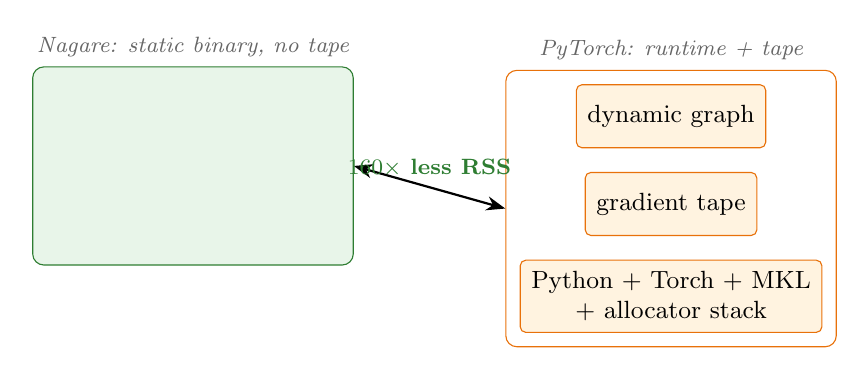
\begin{tikzpicture}[node distance=3mm and 10mm]
  \node[op] (fwd) {forward: straight-line\\closed-form calls};
  \node[op, below=of fwd] (bwd) {backward: hand-derived\\analytic gradients};
  \node[draw=naggreen, fill=lightg, rounded corners, fit=(fwd)(bwd), inner sep=5pt] (nag) {};
  \node[lbl, above=0mm of nag] {Nagare: static binary, no tape};
  \node[op, right=32mm of fwd, fill=lighto, draw=nagorange] (graph) {dynamic graph};
  \node[op, below=of graph, fill=lighto, draw=nagorange] (tape) {gradient tape};
  \node[op, below=of tape, fill=lighto, draw=nagorange] (rt) {Python + Torch + MKL\\+ allocator stack};
  \node[draw=nagorange, rounded corners, fit=(graph)(tape)(rt), inner sep=5pt] (pt) {};
  \node[lbl, above=0mm of pt] {PyTorch: runtime + tape};
  \draw[{Stealth[length=2.4mm]}-{Stealth[length=2.4mm]}, thick]
     (nag.east) -- node[above,font=\footnotesize\bfseries,text=naggreen]{$160\times$ less RSS} (pt.west);
\end{tikzpicture}
\caption{The most robust Nagare advantage is structural: no tape, no runtime.}
\end{figure}

\subsection{The \texttt{ikj}/SAXPY kernel reorder (the big single-kernel win)}
The dominant matmul was a scalar reduction with a \emph{strided} weight load
(Fig.~\ref{fig:ikj} left) --- a strided-gather scalar reduction that LLVM
\textbf{cannot} auto-vectorise. Reordered to \texttt{ikj} (SAXPY) form
(right) --- seed the output row with the bias, then for each input $i$ broadcast
$x_i$ and add a \emph{contiguous} weight row into the \emph{contiguous} output
row --- the inner loop is element-wise over contiguous memory and
\textbf{auto-vectorises to AVX FMA}. It is \textbf{bit-identical} (same summation
order). Measured: \texttt{fused\_update} $\mathbf{2.9\times}$, whole forward
$\mathbf{2.1\times}$, zero accuracy change.

\begin{figure}[h]\centering
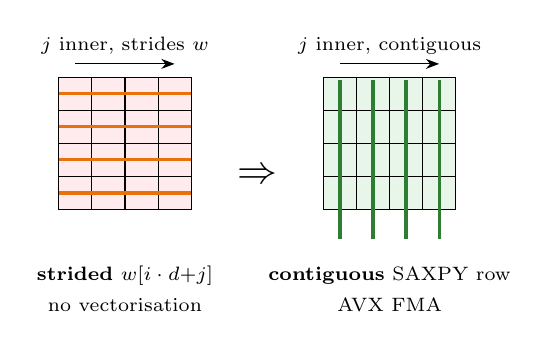
\begin{tikzpicture}[scale=0.42, every node/.style={font=\scriptsize}]
  % strided (bad)
  \foreach \j in {0,...,3}\foreach \i in {0,...,3}
     \draw[fill=lightr] (\i,-\j) rectangle ++(1,1);
  \foreach \j in {0,...,3}\draw[nagorange,very thick] (0,-\j+0.5) -- (4,-\j+0.5);
  \node at (2,-5) {\textbf{strided} $w[i\cdot d{+}j]$};
  \node at (2,-5.9) {no vectorisation};
  \draw[-{Stealth}] (0.5,1.4)--(3.5,1.4) node[midway,above]{$j$ inner, strides $w$};
  % arrow
  \node at (6,-2) {\Large$\Rightarrow$};
  % contiguous (good)
  \begin{scope}[xshift=8cm]
    \foreach \j in {0,...,3}\foreach \i in {0,...,3}
       \draw[fill=lightg] (\i,-\j) rectangle ++(1,1);
    \foreach \i in {0,...,3}\draw[naggreen,very thick] (\i+0.5,0.9) -- (\i+0.5,-3.9);
    \node at (2,-5) {\textbf{contiguous} SAXPY row};
    \node at (2,-5.9) {AVX FMA};
    \draw[-{Stealth}] (0.5,1.4)--(3.5,1.4) node[midway,above]{$j$ inner, contiguous};
  \end{scope}
\end{tikzpicture}
\caption{\label{fig:ikj}The \texttt{ikj} reorder turns a non-vectorisable
strided reduction into a contiguous broadcast-FMA loop --- bit-identical.}
\end{figure}

\subsection{Rayon MapReduce that scales to all cores}
Every row/cycle is independent, so kernels are \texttt{par\_chunks\_mut} over the
output. Decisive on a many-core CPU: \textbf{MKL \emph{oversubscribes} at 32
threads ($4$--$14\times$ \emph{slower} than 8t) while Nagare's rayon scales
cleanly}. At each engine's best thread count, Nagare-CPU beats PyTorch-CPU across
the whole sweep (\S\ref{sec:bench}).

\subsection{Parallel pool (Amdahl), fusion, and Chebyshev-deploy}
After the kernel fix the only serial stage was the pool; on a 32-core box a
serial section dominates (Amdahl), so parallelising it (bit-identical) collapsed
the parity forward $15.7\to7.6$ $\mu$s/sample --- the step that took Nagare from
behind to \emph{beating} PyTorch-CPU. \texttt{fused\_entropy\_update} never
materialises the wide \([h\,|\,\text{pooled}\,|\,\text{ent}]\) broadcast (alloc
halved). The Chebyshev-deploy path (train Catmull--Rom, deploy Chebyshev) is
$1.7$--$1.9\times$ faster than PyTorch at $5$ vs $553$ MiB.

\section{How good it is --- accuracy and AUROC}
The update rule is \emph{local}: $W \mathrel{+}= \eta\,g\,\phi\,(y-p)$, no
reverse-mode into the feature generator.

\begin{table}[h]\centering\small
\begin{tabular}{lcc}
\toprule
task & clean AUROC & hard AUROC (few-shot+noise+missing)\\
\midrule
moons  & $1.000$ & $1.000$\\
spiral & $1.000$ & $0.952$--$0.959$\\
xor    & $1.000$ & $1.000$\\
\bottomrule
\end{tabular}
\caption{Closed-form learner, Mann--Whitney AUROC (\texttt{examples/auroc\_eval.rs}),
$60$ parameters. Clean $=1.0$; robust under heavy corruption; gate-independent.}
\end{table}

The entropy-pool local learner matches a backprop-like baseline's accuracy with
$60$ vs $2{,}836$ parameters ($\sim47\times$ fewer). \textbf{Honest science:} a
point-order-shuffle ablation shows the fitted projection \emph{gate} does not
robustly beat a constant gate; quality comes from the pooled features + the
closed-form update, not the gate mechanism. \textbf{Not yet measured:}
real signed-graph AUROC (Slashdot/Epinions) --- the framework's actual target,
and the decisive next experiment.

\section{Benchmark summary (kato15)}\label{sec:bench}
\begin{figure}[h]\centering
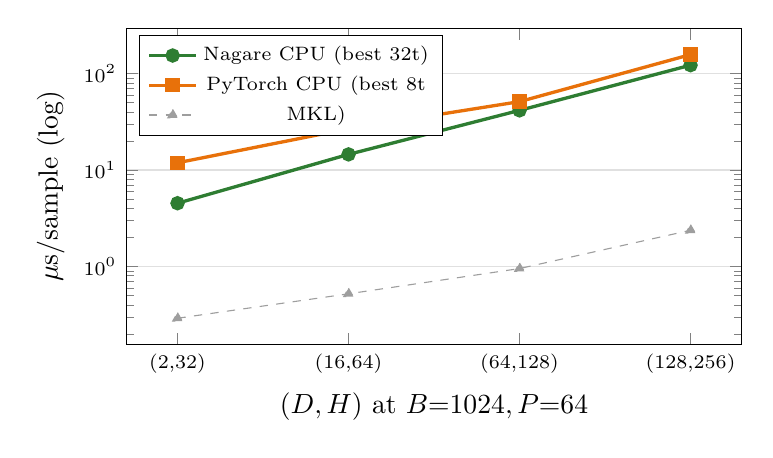
\begin{tikzpicture}
\begin{axis}[width=9.4cm,height=5.6cm,ymode=log,
  xtick={0,1,2,3},xticklabels={{(2,32)},{(16,64)},{(64,128)},{(128,256)}},
  xlabel={$(D,H)$ at $B{=}1024,P{=}64$},ylabel={$\mu$s/sample (log)},
  legend style={font=\scriptsize,at={(0.02,0.98)},anchor=north west},
  ymajorgrids,grid style=black!12, tick label style={font=\scriptsize}]
 \addplot[naggreen,very thick,mark=*] coordinates {(0,4.52)(1,14.50)(2,41.47)(3,121.97)};
 \addplot[nagorange,very thick,mark=square*] coordinates {(0,11.87)(1,26.72)(2,51.09)(3,157.04)};
 \addplot[naggrey,dashed,mark=triangle*] coordinates {(0,0.29)(1,0.52)(2,0.95)(3,2.37)};
 \legend{Nagare CPU (best 32t),PyTorch CPU (best 8t, MKL),CUDA (reference; Nagare GPU = future)}
\end{axis}
\end{tikzpicture}
\caption{Fair CPU-vs-CPU dimensionality scaling: a young closed-form Rust
framework beats a mature MKL-GEMM ecosystem across the whole sweep ($1.2$--$2.6\times$).
The GPU line is a reference ceiling, not a head-to-head (Nagare has no GPU backend
\emph{yet}). Toy-shape forward parity: Nagare $7.6$ vs PyTorch $7.6$--$9.1$; memory
$3$--$160\times$ less throughout.}
\end{figure}

\section{Honest bounds \& roadmap}
\begin{itemize}\itemsep1pt
  \item \textbf{Matched 8 threads, large dense matmul ($D\!\ge\!64$):}
  PyTorch-CPU edges ahead $\sim1.2$--$1.3\times$ --- tuned BLAS blocking/packing.
  Nagare recovers by scaling to all cores.
  \item \textbf{GPU:} a reference ceiling and a defined next step (kernels are
  embarrassingly parallel), not a CPU-vs-GPU verdict.
  \item \textbf{Real-task AUROC} (signed-link prediction) is the next quality
  evidence, and the one that decides whether Nagare is a genuinely different
  \emph{learning} mechanism or a fast lean forward.
\end{itemize}

\paragraph{One line.}\emph{Nagare is fast because it swaps the autograd tape and
tensor-batch dispatch for contiguous, auto-vectorised, closed-form kernels that
MapReduce to every core (where BLAS oversubscribes) --- and good because that
closed-form local learner reaches $\mathrm{AUROC}\approx1.0$ with $\sim47\times$
fewer parameters, on a static binary that uses $3$--$160\times$ less memory.}

\end{document}
